\documentclass{article}

% Language setting
% Replace `english' with e.g. `spanish' to change the document language
\usepackage[english]{babel}
\usepackage[version=4]{mhchem}

% Set page size and margins
% Replace `letterpaper' with `a4paper' for UK/EU standard size
\usepackage[letterpaper,top=2cm,bottom=2cm,left=3cm,right=3cm,marginparwidth=1.75cm]{geometry}

% Useful packages
\usepackage{amsmath}
\usepackage{graphicx}
\usepackage[colorlinks=true, allcolors=blue]{hyperref}

\title{22.01 Fall 2016, Problem Set 1}
\author{Rhett Applestone}
\date{}

\begin{document}
\maketitle


Complete all the assigned problems, and do make sure to show your intermediate work.

\hrulefill

\section{(50 points) Retracing Chadwick’s Discovery of the Neutron}
\begin{enumerate}
    \item What made James first hypothesize an uncharged particle with the mass of a proton?

    Because of the discrepancy between the range of the radiation when aluminum foil was placed between the radiation and the detector, as well as the inability to conserve energy if it was attributed to a high energy photon, he reconciled these by deducing that if there was a particle that would not be affected by the electrons in the foil, and have a mass that would make the equation conserve energy, that would be a valid explanation.
    \item What was the competing hypothesis to explain the observed results?

    The competing hypothesis were either a proton, or a high energy photon as radiation.
    \item Write the nuclear reaction of alpha particles (helium nuclei) bombarding beryllium. You may want
to look up the stable isotope of Be here: http://atom.kaeri.re.kr/

    $$\ce{^4_2\alpha} + \ce{^9_4Be}\xrightarrow{} \ce{^12_6C} + \ce{^1_0n}$$
    \item Why would a neutron have greater “penetrating power” (range) through matter compared to charged
particles? What does a neutron not interact with?

    It wouldn't have any interactions with the electrons which would change the path of any charged particles.
    \item On p. 694 of the second paper, Chadwick states that “The source of polonium was prepared from a
solution of radium by deposition on a disc of silver.” How could polonium be produced directly from
radium?

    Natural radioactive decay from Radium to Polonium which hits Radon as a between stage in the decay chain.
    \item On p. 698 of the second paper, Chadwick states that “the mass of the neutron is equal to that of the
proton...” Is this true? What are the masses of the proton, neutron, and electron? Is the mass of
Rutherford’s “neutron,” consisting of a proton and an electron, equal to the neutron’s mass? Why or
why not (where does the energy discrepancy come from)? Why couldn’t Chadwick discern between
the masses of these two particles?

    The mass of a neutron and a proton are not equal. The mass of a neutron is approximately 1.008664 amu, and the mass of a proton is 1.007276 amu, an electron is 0.00054858 amu.
    The combined mass of a proton and electron is 1.00782458 amu. This is still not the mass of a neutron, however it is closer and within a margin of a thousandth of an amu. It is likely that scientific technology of the time could not differentiate between these small mass differences.   
    \item On pp. 701-702, why is the kinetic energy of 11 B not accounted for, and what does it mean for kinetic
energies to be given in “mass units?” Convert these “mass unit” energies to energies in electron volts
(eV). What is the approximate kinetic energy of 11 B in eV at room temperature?

    Because the rest mass of Boron-11 is likely less than 1/100th of an eV, which can be neglected.
    Mass and energy can be given in interchangeable units via $E=mc^2$ and can be converted with a factor of $931.49\frac{MeVc^2}{amu}$
\end{enumerate}


\section{(50 points) Getting Used to Nuclear Quantities}
In these questions, you will calculate a number of quantities related to nuclear reactions and power generation.
You will have to look up certain reactions and values from primary sources in the literature (books, papers,
databases). Make sure to state which values you look up or assume, and cite your sources using proper
citation methods.
These calculations are useful, especially when arguing the benefits and costs of nuclear power. If you can
derive them quick
\subsection{Relative Power Densities and Nuclear Reactions (15 points)}
Calculate the energy in Joules released from burning 1kg of coal, natural gas, uranium, and deuterium. Use
the CRC Handbook of Chemistry and Physics, available through the MIT Libraries site (libraries.mit.edu), to
find chemical binding energies (otherwise known as enthalpies of formation, or $\Delta$H ) data for your answers. 0
Now repeat this calculation for the nuclear fission of uranium into 90Sr and 145Xe (two typical fission
products), and the nuclear fusion of 2H with 3H. Use the KAERI Table of Nuclides to find the nuclear
binding energies for your answers. Neglect electrons entirely for simplicity.

\vspace{10pt}When looking at the power generated when burning 1kg of coal we must make some assumptions
Firstly, coal is not pure elemental carbon. It comes in many kinds, however according to Reid,

\begin{quote}
    ``Bituminous coal has a composition of about 84.4\% carbon, 5.4\% hydrogen, 6.7\% oxygen, 1.7\% nitrogen, and 1.8\% sulfur, on a weight basis''
\end{quote}


Here I'm just going to focus on the carbon and hydrogen and neglect the others. That means in 1kg of coal you have 0.844kg of carbon and 0.054kg of hydrogen. We also assume that all of the carbon and hydrogen react in their entirety with no losses aswell as at the temperature stated in the CRC Handbook of Chemistry and physics and as gasses.\vspace{10pt}

$$C+O_2\xrightarrow{}CO_2+Energy$$
$$2H_2+O_2\xrightarrow{}2H_2O+Energy$$


\begin{center}
    Energy from just carbon
\end{center}
$$\left(\frac{0.844 \ kg \ of \ C}{1}\right)\left(\frac{1u}{1.660540\times10^{-27}kg}\right)\left(\frac{1 \ atom \ of \ C}{12.011u}\right)\left(\frac{1 \ mol}{6.02214076\times10^{23}\ particles}\right)\left(\frac{393.51kJ}{1 \ mol}\right)= 27.7MJ$$\vspace{10pt}
\
\begin{center}
    Energy from just hydrogen
\end{center}

$$\left(\frac{0.054 \ kg \ of \ H}{1}\right)\left(\frac{1u}{1.660540\times10^{-27}kg}\right)\left(\frac{1 \ atom \ of \ H}{1.008u}\right)\left(\frac{1 \ mol H}{6.02214076\times10^{23}\ particles}\right)\left(\frac{1mol
H_2O}{2 \ mol H}\right)\left(\frac{285.830kJ}{1 \ mol H_2O}\right)$$\vspace{10pt}
$$=7.7MJ$$

\begin{center}
    and together we get that one kg of coal has around 35.4MJ of energy if burned entirely with no losses
\end{center}\vspace{10pt}

For natural gas, or methane the calculations are as follows \vspace{10pt}
$$CH_4+2O_2\xrightarrow{}CO_2+2H_2O+Energy$$

We need to know first the binding energy of the $CH_4$ because it will be broken, then we need to know the binding energies of the $CO_2$ and $H_2O$ as they are formed so we can solve for the extra energy. We are neglecting the binding energy of $O_2$ here\vspace{10pt}

To make things simpler lets figure out how much energy is just released from 1 mol of $CH_4$ then figure out how many mols of $CH_4$ there are in one kg of the substance and multiply

it takes $\frac{74.6 \ Kj}{mol}$ to break the $CH_4$, and the $CO_2$ formed releases $\frac{393.51 \ kj}{mol}$ and because in the reaction for each molecule of $CH_4$ put in, you get two of $H_2O$ out, we multiply the binding energy of $H_2O$ by two, which comes out to $2(\frac{285.83kj}{mol})$ If we figure out the final difference in energy per mol of methane we find that it is $\frac{890.57kj}{mol}$ this number will hopefully make calculations much easier\vspace{10pt}

Now, how many mols of methane are there in 1kg of methane, and how many joules are released by burning it?\vspace{10pt}

$$\left(\frac{1 \ kg \ of \ CH_4}{1}\right)\left(\frac{1u}{1.660540\times10^{-27}kg}\right)\left(\frac{1 \ molecule \ of \ CH_4}{16.043u}\right)\left(\frac{1 \ mol}{6.02214076\times10^{23}\ particles}\right)\left(\frac{890.57kJ \ released}{1 \ mol \ CH_4}\right)$$\vspace{10pt}

$$=55.511MJ$$\vspace{10pt}

(not sure why, but this is about 5MJ difference from the answer key)\vspace{10pt}

Next, 1kg of uranium. Didn't know Uranium could burn in air, but I assume the reaction goes as such

$$U + O_2 \xrightarrow{} UO_2 + Energy$$\vspace{10pt}

\begin{center}
    The calculations are pretty similar to the others
\end{center}\vspace{10pt}

$$\left(\frac{1\ kg \ of \ U}{1}\right)\left(\frac{1u}{1.660540\times10^{-27}kg}\right)\left(\frac{1 \ atom \ of \ U}{238.03u}\right)\left(\frac{1 \ mol}{6.02214076\times10^{23}\ particles}\right)\left(\frac{1085.0kj}{1 \ mol}\right)= 4.5582 MJ$$\vspace{10pt}
\begin{center}
    Now on to Deuterium\vspace{10pt}
\end{center}


$$4D + O_2 \xrightarrow{} 2D_2O + Energy$$

$$\left(\frac{1\ kg \ of \ D}{1}\right)\left(\frac{1u}{1.660540\times10^{-27}kg}\right)\left(\frac{1 \ atom \ of \ D}{2.01410u}\right)\left(\frac{1 \ mol}{6.02214076\times10^{23}\ particles}\right)\left(\frac{249.20kj}{1 \ mol}\right)=123.73MJ$$\vspace{10pt}
\begin{center}
    Nuclear fission of uranium into 90Sr and 145Xe 
\end{center}\vspace{10pt}
$$^1_0n + ^{235}_{92}U \xrightarrow{} ^{90}_{38}Sr + ^{145}_{54}Xe + ^1_0n$$\vspace{10pt}
 

I will assume that the incoming and outgoing neutron will have similar Ke, so they will not be considered during calculations. This means that the energy released will be the differences in mass from initial U-235 and the two products will be however much energy is released. \vspace{10pt}

$$235.043928117u-(89.90772787u+144.944719631u) = 0.191480616u$$

This means with each fission there is 0.191480616 amu of mass turned to energy\vspace{5pt}

next we just find out how many atoms there are in a 1kg chunk of U-235 and multiply across\vspace{10pt}

$\left(\frac{1 \ kg \ of \ U-235}{1}\right)\left(\frac{1u}{1.660540\times10^{-27}kg}\right)\left(\frac{1 \ atom \ of \ U-235}{235.043928117u}\right)\left(\frac{ 0.191480616 amu \ released}{1 \ atom \ U-235}\right)\left(\frac{1.4923933\times10^{-10} J}{1 amu}\right)$\vspace{10pt}

$$=7.321663\times10^{13}J$$\vspace{10pt}

For the fusion of Deuterium and Tritium we assume that the 1kg of both is split in equal numbers to have no eccess in the reaction\vspace{10pt}

$$^2_1H+^3_1H\xrightarrow{} ^4_2He + ^1_0n + Energy$$

for this reaction we must find how much energy is released, and how many of these reactions could happen

$$(M_1+M_2)-(M_3+M_4)= (2.014102u+3.016049u)-(4.002603u+1.008665u)= 0.018883u \ of \ M\xrightarrow{}E$$

In 1kg of Deuterium tritium gas there would be \vspace{10pt}
$$\left(\frac{1kg \ D+T}{1}\right)\left(\frac{1u}{1.660540\times 10^{-27}kg}\right)\left(\frac{pairs \ of D+T}{5.030151u}\right)\left(\frac{0.018883u \ converted}{Pair \ of \ D+T}\right)\left(\frac{1.4923933\times10^{-10} J}{1 amu}\right)$$\vspace{10pt}

$$=3.3738 \times 10^{14} J$$

(answer key says to the power of 15, but I believe that may be an error, unless I messed up an exponent somewhere)\vspace{10pt}





 Reid, William (1973). "Chapter 9: Heat Generation, Transport, and Storage". In Robert Perry; Cecil Chilton (eds.). Chemical Engineers' Handbook (5 ed.).\vspace{10pt}

 \
Values for amu of carbon taken from ptable \href{https://ptable.com/}{https://ptable.com/}

\vspace{10pt}

heavy water binding energy taken from nist 
\href{https://webbook.nist.gov/cgi/cbook.cgi?ID=C7789200&Mask=6F}{https://webbook.nist.gov/cgi/}
\subsection{Accelerator Energetics (20 points)}
A common tool to provide data on nuclear reactions and to perform irradiations is the electrostatic accelerator. These work by accelerating charged particles through a large, static electric field. We consider here an
W n accelerator that provides a 1.7MV potential drop over 2m for doubly charged iron ions F e+2 , which enter
the accelerator at ˜zero kinetic energy into the accelerator from an ion source.\vspace{10pt}




\subsubsection{What will be the kinetic energy of an iron ion in eV, as it exits the accelerator?}

If we know one electron moving across a one volt potential difference is equal to an eV, this iron ion with a charge of 2+ should have a KE of 3.4 MeV leaving the accelerator.

\subsubsection{What will be its total mass (not its rest mass) as it exits the accelerator?}\vspace{10pt}

Conv energy to mass and add to atomic mass

$$\left(\frac{1u}{931.49MeVc^2}\right)\left(\frac{3.4MeV
}{1}\right) + 55.934935537u = 55.938585603u$$

\subsubsection{If the ion source injects 2mA of current, what is the total number of particles leaving
the accelerator per second?}

Current is a measure of charges/second, measured in columbs. This means if we have 2mA of current on for one second, we would have 2mC. Each particle is 2+, so it carries two extra positive charges\vspace{10pt}

$$\left(\frac{2\times10^{-3}C}{1}\right)\left(\frac{e}{3.2\times10^{-19}C}\right)=6.25\times10^{15} \ particles \ per \ second$$
\subsubsection{What is the total power, in Watts, associated with pulling 2mA of current through
1.7MV of electrostatic potential? Where does this power go?}\vspace{10pt}

$P=IV, (2\times10^{-3}A)(1.7\times10^6V)=3.4KW$ \vspace{10pt}

The power would be transfered to the particles that are being 
accelerated\vspace{5pt}

(Key says dissipated as heat as they hit the target, which makes sense)


Here is a picture of DANTE, the accelerator in question. It lives in the basement of NW13.

\begin{center}
    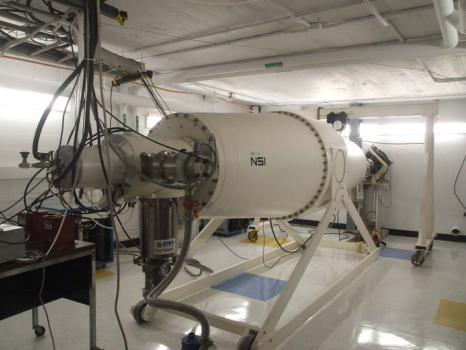
\includegraphics[scale=0.5]{dante.png}
\end{center}




\subsection{Mass-Energy Equivalence (20 points)}
From special relativity, the total mass (m) of a moving particle can be expressed as follows:

$$m = \frac{m_0}{\sqrt{1-\frac{v^2}{c^2}}}= \gamma m_0 \ \ \ \ \ \gamma = \frac{1}{\sqrt{1-\frac{v^2}{c^2}}}$$

where $m_0$ is it's rest mass and, v is it's velocity, and c is the speed of light.

\subsubsection{What is the particle's mass at the following speeds:  $\frac{1m}{s}$, 1 $\frac{1km}{s}$, 0.9c, 0.99c, c?}\vspace{10pt}

The mass of an $^{56}Fe^{2+}$ ion at rest would be 55.933838377u. At 1m/s it's mass would be \vspace{10pt}

$$m = \frac{55.933838377u}{\sqrt{1-\frac{(1m/s)^2}{(299792458m/s)^2}}}$$ which is effectively the same as it's rest mass\vspace{10pt}

at 1km/s
$$m = \frac{55.933838377u}{\sqrt{1-\frac{(1000m/s)^2}{(299792458m/s)^2}}}=55.9338383773u$$
Still almost no change\vspace{10pt}

at 0.9c
$$m = \frac{55.933838377u}{\sqrt{1-\frac{(269813212.2m/s)^2}{(299792458m/s)^2}}}=128.321025899u$$ or a bit over double\vspace{10pt}


$$m = \frac{55.933838377u}{\sqrt{1-\frac{(296794533.42m/s)^2}{(299792458m/s)^2}}}=396.504466923u$$ or about 7.08x the original mass\vspace{10pt}

at c mass goes to $\infty$


\subsubsection{ Derive an expression for the particle’s kinetic energy (T) in terms of its total and rest
masses.}\vspace{10pt
}

$$T=\frac{1}{2}mv^2 \And m = \frac{m_0}{\sqrt{1-\frac{v^2}{c^2}}}$$
$$\sqrt{1-\frac{v^2}{c^2}} = \frac{m_0}{m}$$
$$1-\frac{v^2}{c^2} = (\frac{m_0}{m})^2$$
$$1-(\frac{m_0}{m})^2 = \frac{v^2}{c^2}$$
$$c^2(1-(\frac{m_0}{m})^2) = v^2$$
$$T=\frac{1}{2}mc^2(1-(\frac{m_0}{m})^2)$$

(not sure if that is correct, the answer key has a much simpler explanation)\vspace{10pt}

Say a particle's total energy is equal to $T+E_0$ It's total energy is also equal to $\gamma m_0c^2$, $E_0$ can be written as $m_0c^2$, and we are able solve for T as such. \vspace{10pt}

$$T+E_0=\gamma m_0c^2$$
$$T+m_0c^2=\gamma m_0c^2$$
$$T=\gamma m_0c^2-m_0c^2$$
$$T=(\gamma-1)m_0c^2$$

\subsubsection{Show that the particle’s momentum (p) can be described in terms of its kinetic energy
and rest mass as follows:}

$$p = \frac{1}{c}\sqrt{T^2 + 2Tm_0c^2}$$

Start with the total relativistic energy of a moving particle:

$$ E=\sqrt{p^2c^2+E^2_{rest mass}}$$

$$ \gamma m_0c^2=\sqrt{p^2c^2+E^2_{rest mass}}$$
$$ T + m_0c^2=\sqrt{p^2c^2+E^2_{rest mass}}$$
$$ (T + m_0c^2)^2=p^2c^2+E^2_{rest mass}$$
$$ (T + m_0c^2)^2=p^2c^2+(m_0c^2)^2$$
$$ (T + m_0c^2)^2-(m_0c^2)^2=p^2c^2$$
$$ \frac{(T + m_0c^2)^2-(m_0c^2)^2}{c^2}=p^2$$
$$ \sqrt{\frac{(T + m_0c^2)^2-(m_0c^2)^2}{c^2}}=p$$
$$ \sqrt{\frac{T^2 + 2Tm_0c^2+m_0^2c^4-m_0^2c^4}{c^2}}=p$$
$$ \sqrt{\frac{T^2 + 2Tm_0c^2}{c^2}}= \frac{1}{c}\sqrt{T^2 + 2Tm_0c^2} = p$$









\subsubsection{Radioactive decay typically proceeds with the emission of ˜1 MeV particles. For the
case of an alpha particle, a beta particle, a neutrino, and a neutron of kinetic enregy
1 MeV, which ones must be treated in a relativistic manner? You will have to look up
the rest masses of each particle in your answer. Note that the neutrino was only proven
to have mass last year!}\vspace{10pt}

I define any mass increase over one percent to be relevant to relativistic calculations. This happens at around 0.14c or 42000000 m/s\vspace{10pt}

converting Mev to J we get $1.60218*\times10^{-13}J$ of KE for each particle.\vspace{10pt}

For $^4_2\alpha$ $$\sqrt{\frac{2T}{m_0}}=V= \sqrt{\frac{3.20436\times10^{-13}J}{6.644660\times10^{-27}kg}}=6.64465\times10^6m/s$$ which means it's not going to be affected in any meaningful way by relativity\vspace{10pt}

For a $\beta$ particle, or electron $$\sqrt{\frac{2T}{m_0}}=V= \sqrt{\frac{3.20436\times10^{-13}J}{9.1093837\times10^{-31}kg}}=$$ When doing this you get a number that is a multiple of C, which means you probably shouldn't use the logic of $T=\frac{1}{2}mv^2$ and we have to adopt a new strategy.\vspace{10pt}

(Looked at key for guidance)\vspace{5pt}

Let's use gamma as our new defining variable. Anything over 1.01 is relevant to relativistic treatment


Let's try again for the $\beta$ particle
$$T=(\gamma-1)m_0c^2$$
$$\frac{T}{m_0c^2}+1=\gamma$$
$$\frac{1Mev}{0.511MeV}+1=\gamma=2.95$$ Which we define as significant to relativistic calculations\vspace{10pt}


Since the mass of a neutrino is less than that of a beta particle, and since we already established that a beta particle would need relativistic consideration, it is clear that a neutrino will aswell.\vspace{10pt}


For a neutron the calculations are as follows
$$\frac{T}{m_0c^2}+1=\gamma$$
$$\frac{1mev}{940.6MeV}+1=\gamma=1.001$$ which we do not consider worthy of relativistic calculations.




\
\
\

MIT OpenCourseWare
\href{https://ocw.mit.edu}{https://ocw.mit.edu}

\

22.01 Introduction to Nuclear Engineering and Ionizing Radiation
Fall 2016


For information about citing these materials or our Terms of Use, visit: 

\href{https://ocw.mit.edu/terms}{https://ocw.mit.edu/terms}
\end{document}